% !TEX root = ../../mythesis.tex

\chapter{Background}
\label{chap:background}
    This chapter reviews the necessary background knowledge for the reader to be better acquanited with the work conducted within this thesis.
    It highlights the foundational technical basics of Ethereum blockchain, smart contracts and the most common vulnerabilities associated with smart contracts.
    We cover these technicalities in the following order (based on the work of~\cite{ferreira2022smart}):
        First, we go over the basics of Ethereum, its components and structure. We will go through how blocks are formed,
        what sort of accounts exist on the Ethereum network, and how transactions are executed.
        We will also go through how the Ethereum Virtual Machine functions.
        Afterwards, we will go over smart contracts and their most common vulnreabilities out in the wild.
        We will discuss Solidity-written source code and bytecode of smart contracts, and explain each vulnrability according to the DASP 10 classification.~\cite{dasp}


\section{Ethereum}
    Ethereum is a decentralized virtual machine that was introduced as an alternative blockchain technology to Bitcoin in 2014 by~\cite{wood2014ethereum}.
    A blockchain is essentially a peer-to-peer network made up of computers that act as nodes and distribute updates for a single database without necessarily having confidence in one another.
    It is based on a combination of combination of cryptography, networking, and incentive mechanisms.~\cite{wohrer2018smart}
    The aforementioned database effectively serves as a ledger, recording each and every transaction that each node in the blockchain network makes. 


    \begin{figure}
        \centering
        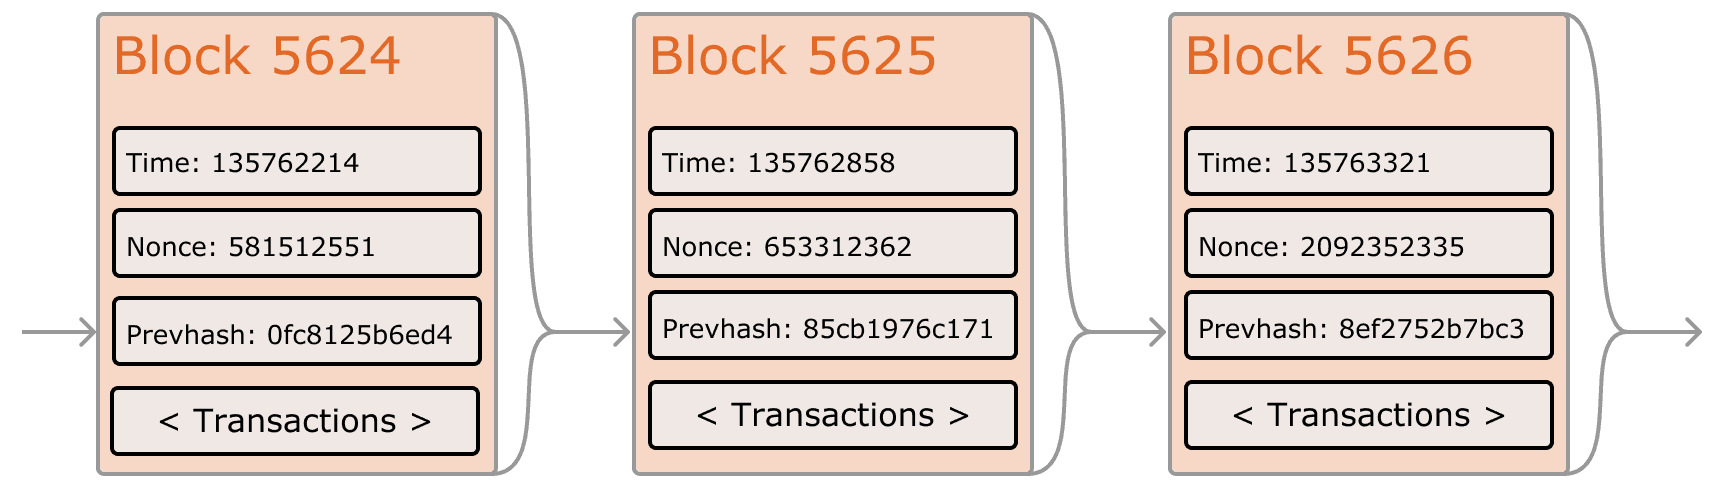
\includegraphics[width=\textwidth]{figures/ethereum-blocks.png}
        \caption{Ethereum blockchain structure.}
        \label{fig:ethereumBlockchainStructure}
    \end{figure}

    As the second most popular blockchain, the Ethereum blockchain was developed as an alternative to cover for the lackings of Bitcoin.
    It is a transaction-based, cryptographically secure state machine, that reads a series of inputs and, based on those inputs, transitions to a new state.~\cite{ferreira2022smart}
    Just like Bitcoin, Ethereum currently uses Proof-of-Work (PoW) as its consensus protocol.
    Proof-of-Stake (PoS), PBFT(Practical Byzantine Fault Tolerance), and DPoS (Delegated Proof of Stake) are other forms of concensus protocol, for example.
    The solution to a series of cryptographic puzzles are used in the PoW mechanism to prove the credibility of the data being written on the blockchain, using such mechanism as their consensus protocol.
    The puzzle is usually a computationally hard but easily verifiable mathematical problem.
    When a node creates a block, it must resolve a PoW puzzle and spend computing power to achieve so. The nodes compete o=with each other over this objective function and the node with the most computing power usually succeeds ind doing so.
    After the PoW puzzle is resolved, it will be broadcasted to other nodes, so as to achieve the purpose of consensus and append a new block to the blockchain.
    It acts as a “proof” that a node has done “work” by spending its computational resources.
    This process is known as mining and nodes which decide to participate in this process and try to create new blocks are known as miners.

    \begin{figure}
        \centering
        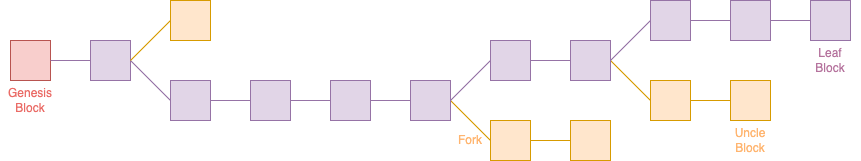
\includegraphics[width=\textwidth]{figures/uncle.png}
        \caption{An illustration of Ethereum's GHOST protocol.}
        \label{fig:uncle}
    \end{figure}

    \subsection{Ether}

    \subsection{Accounts}
        The Ethereum state is consisted of many small objects naemd as accounts, where each account has a 20-byte address and state transitions to be able to interact with the other accounts on-chain.
        An address on the Ethereum blockchain is a 160-bit identifier that is used to identify any account.
        The world state is a mapping between addresses and account states.~\cite{wood2014ethereum}
        Ethereum suppotrs two types of accounts: externally owned
        (controlled by private keys) -namely EOA's- and contract accounts (CA'S, controlled by their contract code)~\cite{ethereum2014ethereum}.
        Inside of an Ethereum account is composed of four fields: nonce, ether balance, contract code hash, and storage root, explained as follows:

        \begin{itemize}
            \item \textbf{Nonce:} Nonce represents the number of transactions sent from particular address or the number of contract creations made by an account and is used as a guarantee that each transaction can only be processed once.
            \item \textbf{Balance:} Ether balance is the number of Wei owned by this address
                Wei is the smallest subunit of ether (1 wei is equivalent to 10-18 ether).
            \item \textbf{Storage Root:} Storage root is the 256-bit hash of the root node of a Merkle Patricia tree that represents the content of the account 
            \item \textbf{Contract CodeHash:} Contract code hash is the Keccak-256 hash of Ethereum Virtual Machine (EVM) code of the account, which is executed if an address receives a message call.
        \end{itemize}

    \subsection{Transactions}
        Transactions are essentially cryptographically signed instructions from EOAs to update the state of the Ethereum blockchain.
        EOAs sign their transactions using their private key in order to cryptographically prove that the transaction could only have come from them and not from someone else.
        Two types of transactions exist: message calls and contract creations.
        The latter are transactions with an empty recipient field that result in creating new CAs (i.e., smart contracts). 
        The code, to be associated with the CA, is placed inside the data field of the transaction.
        Regardless of their type, all transactions contain the following fields:
            \begin{itemize}
                \item A count on the number of transactions sent by the sender. This number is incremented by one every time a transaction is sent by the sender.
                \item The amount of wei that the sender is willing to pay for each unit of gas that is used during the execution of the transaction.
                \item The maximum amount of gas units that the sender is willing to spent for the execution of this transaction.
                    This amount is set and paid upfront, before any computation is performed.
                \item The address of the recipient. If the recipient is an EOA, the transaction will transfer value, if the recipient is a CA, the transaction will transfer value as well as
                execute the contract's code.
                    A transaction with an empty recipient address is used to trigger the creation of a new CA.
                \item The amount of wei to be sent from the sender account to the recipient account.
                    Interestingly, this value may be used to set the starting balance of the newly created CA in a contract-creating transaction.
                \item These values represent the digital signature (R, S) which can be used to recover the public key (V).
                    These values identify the sender of the transaction and confirms that the sender has authorized the transaction.
                \item This field is only part of contract-creating transactions and consists of an unlimited length byte array that includes the code to be used during the initialization process
                and the code to be permanently associated with the newly created CA.
                \item This is an optional field that is only part of message calls and consists of a byte array of unlimited size that specifies the input data (e.g., , function name, function parameters)
                of the message call.
            \end{itemize}

    \subsection{Blocks}
        Every Blockchain, including Ethereum, consists of a sequence of blocks, which are bound and "chained" together through cryptographic hashes, grouping transactions altogether.
        A block on the Ethereum blockchain consists of a body and a header.
        The block header contains metadata about its own specific block. 
        The first block of the Blockchain is called genesis which has no parent block.
        An ommer is a block whose parent is equal to the current block's parent's parent.
        A block header is a portion of the block consisting of the following apart from the transactions listed inside:

        \begin{itemize}
            \item \textbf{ParentHash}: This is the Keccak-256 hash of the parent block's header.
            \item \textbf{OmmersHash}:This is the Keccak-256 hash of the ommer's list portion of this block.
            \item \textbf{Beneficiary}: The account address that receives the fees for mining this block
            \item \textbf{LogsBloom}: A Bloom filter (i.e., a data structure) that allows efficient querying of information contained in the logs.
            \item \textbf{Difficulty}: the diKculty level of this block, i.e. the required effort for mine a block.
            \item \textbf{Number}:  the count of current block (the genesis block has a block
            number of zero; the block number increases by 1 for each each
            subsequent block)
            \item \textbf{GasLimit}: The current gas limit per block.
            \item \textbf{GasUsed}: the sum of the total gas used by transactions in this block.
            \item \textbf{ExtraData}: Arbitrary data that can set by the miner. This data is limited to 32-byte and usually refers to the name of the miner or the client version that was used to
            mine the block.
            \item \textbf{StateRoot}: the hash of the root node of the state trie (recall how we
            learned that the state trie is stored in the header and makes it easy
            for light clients to verify anything about the state)
            \item \textbf{Timestamp}: The UNIX timestamp when the block was mined.
            \item \textbf{Nonce}: A hash that, when combined with the mixHash, proves that this block has carried out enough computation
            \item \textbf{MixHash}: A hash that, when combined with the nonce, proves that
            this block has carried out enough computation
            \item \textbf{TransactionsRoot}: The hash of the root node of the Merkle Patricia trie that stores all transactions listed in this block.
            \item \textbf{ReceiptsRoot}: The hash of the root node of the Merkle Patricia trie that stores the receipts of all transactions listed in this block.
                Transaction receipts are generated after the execution of a transaction contain information such as logs or the actual gas that has been used during execution.

        \end{itemize}

    \subsection{Ethereum Virtual Machine}
        The formal definition of the EVM is specified in the Ethereum Yellow Paper.~\cite{wood2014ethereum}
        The Ethereum Virtual Machine (EVM) at the heart of the Ethereum blockchain is a VM (virtual machine), with a stack-based architecture with 256-bit word sizes, supporting Turing-complete programming languages.
        EVM handles the computation side for Ethereum and comes with a set of instructions (namely, opcodes).
        Thus, a smart contract from a low-level point of view is a series of opcode instructions which EVM can read and compute and execute the logic of that smart contract.
        The EVM is also responsible for handling the estimation and calculation of gas consumption for transactions in smart contracts.

\section{Smart Contracts}
    The concept of smart contracts - programs running on the EVM - has been first introduced by Nick Szabo in one of his works in 1997.~\cite{szabo1997formalizing}
    They provide a framework that allow any sound program to be executed in an autonomous, distributed, and trusted manner.~\cite{nguyen2020sfuzz}
    The main programming langauge currently in use for the development of smart contracts is Solidity, although Vyper is gaining gradual traction as well.

    \subsection{Vulnerabilities}
        Solidity, like any other programming langauge in history, is prone to all kinds of vulnreabilities.
        What makes security vulnerabilities in Solidity so attractive is the fact that the programs written in Solidity are very much often used in the financial sector,
        handling millions of dollars in digital aassets and cryptocurrencies. Attcking such contracts successfully can result in enormous financial losses.
        Some of these vulnerabilities like another programming language arise from the human factor invlved in development of the smart contracts, and some specific to the blockchain data structuresa and how they and their components function and interact with each other.
        And these are only vulnerabilities at the scope of smart contracts we are focusing on. Vulnerabilities can arise with regards to core infrastructure of the blockchains handling smart contracts as well.
        In this section, we go over 9 of the more discussed vulnerabilities in Solidity and Ethereum according to ~\cite{dasp} to get a better sense of what threat surface the deveopers and researchers developing analysis tools face:

            \paragraph{Re-entrancy}
            Often called as the most famous Ethereum vulnerability, the re-entrancy attack has been a great example at showing the risks of \textit{"Code is Law"} and the importance of smart contract security, historically.
            The DAO hack ~\cite{dhillon2017dao} is one of the most famous real worl examples of the re-entrancy hack.
            The re-entrancy attack can also be counted as a type of denial-of-service (DoS) attack, where a malicious actor can cause a program to infinitely loop and consume CPU cycles and in the case of smart contracts, drain a wallet of its ETH's.
            Reentrancy occurs when external contract calls are allowed to make new calls to the calling contract before the initial execution of that call is complete.
            For a function, this means that the contract state may change in the middle of its execution as a result of a call to an untrusted contract. ~\cite{dasp}

            \paragraph{Access Control}
            The Access Control vulnerability, not exclusive to smart contract types of programs, usually occur when smart contracts use use poor visibility settings with regards to calling functions.
            This gives the attackers the ability to try to access the smart contract's private values, or hijack the control of the smart contract (for example, becoming the owner of a contract by initializing that contract through a statement like \texttt{owner = msg.sender()}).

            \paragraph{Arithmetic}
            Integer overflows and underflows can cause huge losses in smart contract-based applications~\cite{arithmeticVuln}.
            Values assigned with the integer data type, if not handled carefully with regard to being signed or unsigned integers, can cause overflows and underflows and cause DoS-type attacks.
            
            \paragraph{Unhandled Exception}
            Also known as unchecked-send, this vulnerability  can cause unwanted outcomes when the smart contract is executed, due to the fact that some low level calls in Solidity like \texttt{call()} and \texttt{delegatecall()} can return a boolean value set to the value False and lt the execution flow resume if an error happens mid-execution.
            This is not ideal since it means that the execution of the smart contract has not been reversed and has successfully been completed, but with wrong or undesirable outcomes.
            Thus, the return values of such low-level calls should always be checked and the develoeprs need to make sure that such exceptions are handled appropriately during execution.
            
            \paragraph{Frontrunning}
            The frontrunning vulnerability is one of the more famous ones in the list, also known as Transaction Ordering Dependance (TOD).
            Explotation of this vulnerability happens when malaicious miners decide to alter the initial default ordering of the transactions submitted to the blockchain.
            Per Eskandari et al.~\cite{eskandari2018frontrunning}, frontrunning can be generally reduced into three templates:
            \begin{itemize}
                \item Displacement attack, where an adversarial party makes a transaction in order to displace the victim user's transaction by having a higher gas price and thus, the attacker's tarnsaction gets mined before that of victim's due to it giving having more aligned incentives with he miners' network.
                \item Insertion attack, in which an adversary makes two transactions, one with a higher gas price than the victim transaction and one with a lower gas price, to \textit{sandwich} the victim transaction.~\cite{varun2022mitigating}
                \item Supperession attack, where an attacker makes multiple transactions with higehr gas prices that the victim transactions to prevent them from being mined in the same block.
            \end{itemize}

            \paragraph{Bad Randomness}
            Also known as \textit{nothing is secret},~\cite{dasp} this vulnerability happens when smart contracts attempt to generate random, or to be more exact, pseudo-random numbers for any number of reasons.
            If the smart contract generating the pseudo-random number computes that random number using values that can be guessed by a malicious party, then the attacker can predict the next number that will be generated.
            Values such as block timestamps,or block number are generally advised against to be used in such mechanisms. They are called hard-to-predict values but it is better to use an external oracle to generate the random numbers needed~\cite{swcregistry}.
        
            \paragraph{Time Manipulation}
            This vulnerability is also known as \textit{timestamp dependence}~\cite{dasp}.
            In Solidity, a block's timestamp is often used to generate psuedi-random numebrs and in other times, it can be leveraged for smart contracts to conduct time-intesive oeprations, like unlocking funds at a specific time.
            A malicious miner of a block can manipulate the timestamp reported while generating the block and sue this vulenrability to their own profit. 
        
            \paragraph{Short Address}
            The short address vulnerability, also known as off-chain issues, results from the Ethereum Virtual Machine accepting arguments with incorrect paddings.
            Attackers trying to exploit this vulnerability, can craft truncated addresses which clients may encode incorrectly in transactions.
            Additioally, it has not been exploited in the wild as mentioned by ~\cite{ferreira2020smartbugs}.